\section*{Задача 3.3}
Дана система уравнений $Ax = b$ c матрицей $A$ из задачи 3.2 и вектором $b:\ b_i = |N - 25| + 5$, где N - номер варианта. Решить систему методом Якоби с точностью $\varepsilon = 10^{-10}$.

\subsection*{Решение}
1. Составим программу преобразования системы $Ax = b$ к виду $x = Bx + c$.

\begin{verbatim}
def Jacobi(A, b):
    '''Перобразует СЛАУ Ax=b к виду x = Bx + c.'''
    B = np.zeros_like(A)
    c = np.zeros_like(b)
    for i in range(A.shape[1]):
        B[i, :] = -A[i, :] / A[i, i]
        B[i, i] = 0
        c[i,0] = b[i,0] / A[i, i]
    return B, c
\end{verbatim}

Убедимся, что выполнено достаточное условие сходимости метода: $||B|| < 1$
\begin{verbatim}
B, c = Jacobi(A, b)
np.linalg.norm(B)

0.6428766787355629
\end{verbatim}

2. Составим программу метода простых итераций с подсчетом нормы вектора невязки на каждой итерации.
\begin{verbatim}
def MPI(A, b, eps):
    B, c = Jacobi(A, b)
    x0 = c
    x1 = B.dot(x0) + c
    iters = 1
    r_n = []
    k = (1 - inf_norm(B)) / inf_norm(B)
    while inf_norm(x1 - x0) > k * eps:
        r_n.append(euclid_norm(A.dot(x1) - b))
        x0 = x1
        x1 = B.dot(x1) + c
        iters +=1
    print("Выполнено итераций: ", iters)
    return x1, np.array(r_n)
\end{verbatim}

Убедимся, что выполнено достаточное условие сходимости метода: $||B|| < 1$.
\begin{verbatim}
B, c = Jacobi(A, b)
np.linalg.norm(B)

0.6428766787355629
\end{verbatim}

Составим программу метода простых итераций с подсчетом нормы вектора невязки на каждой итерации.
\begin{verbatim}
def MPI(A, b, eps):
    B, c = Jacobi(A, b)
    x0 = c
    x1 = B.dot(x0) + c
    iters = 1
    r_n = []
    k = (1 - inf_norm(B)) / inf_norm(B)
    while inf_norm(x1 - x0) > k * eps:
        r_n.append(euclid_norm(A.dot(x1) - b))
        x0 = x1
        x1 = B.dot(x1) + c
        iters +=1
    print("Выполнено итераций: ", iters)
    return x1, np.array(r_n)
\end{verbatim}

Найдем решение задачи с заданной точностью.

\begin{verbatim}
x, r_n = MPI(A, b, eps)

Выполнено итераций:  13
\end{verbatim}

Подставим найденое решение в исходное уравнение и убедимся в корректности метода:
\begin{verbatim}
A.dot(x).T

array([[8., 8., 8., 8., 8., 8., 8., 8., 8., 8., 8., 8., 8., 8., 8., 8.,
        8., 8., 8., 8.]])
\end{verbatim}

Нормы векторов невязки по итерациям:

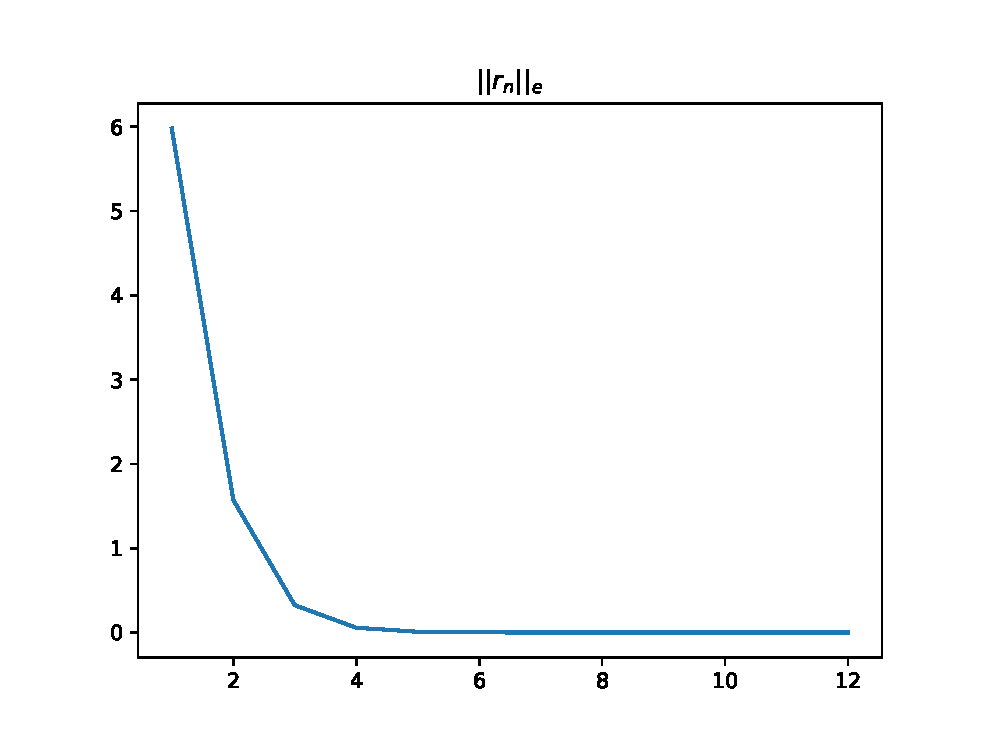
\includegraphics[width=15cm]{fig331.eps}
